\documentclass{article}

\usepackage{graphicx}
\usepackage{tikz}
\usepackage{tikzsymbols}
\usetikzlibrary{calc,patterns,shapes.geometric}
\pagestyle{empty}
\usepackage[margin=0pt]{geometry}
\geometry{papersize={14in,12in}}

\def\centerarc[#1](#2)(#3:#4:#5){\draw[#1] ($(#2)+({#5*cos(#3)},{#5*sin(#3)})$) arc (#3:#4:#5);}

\begin{document}
	\begin{figure}
		\centering
		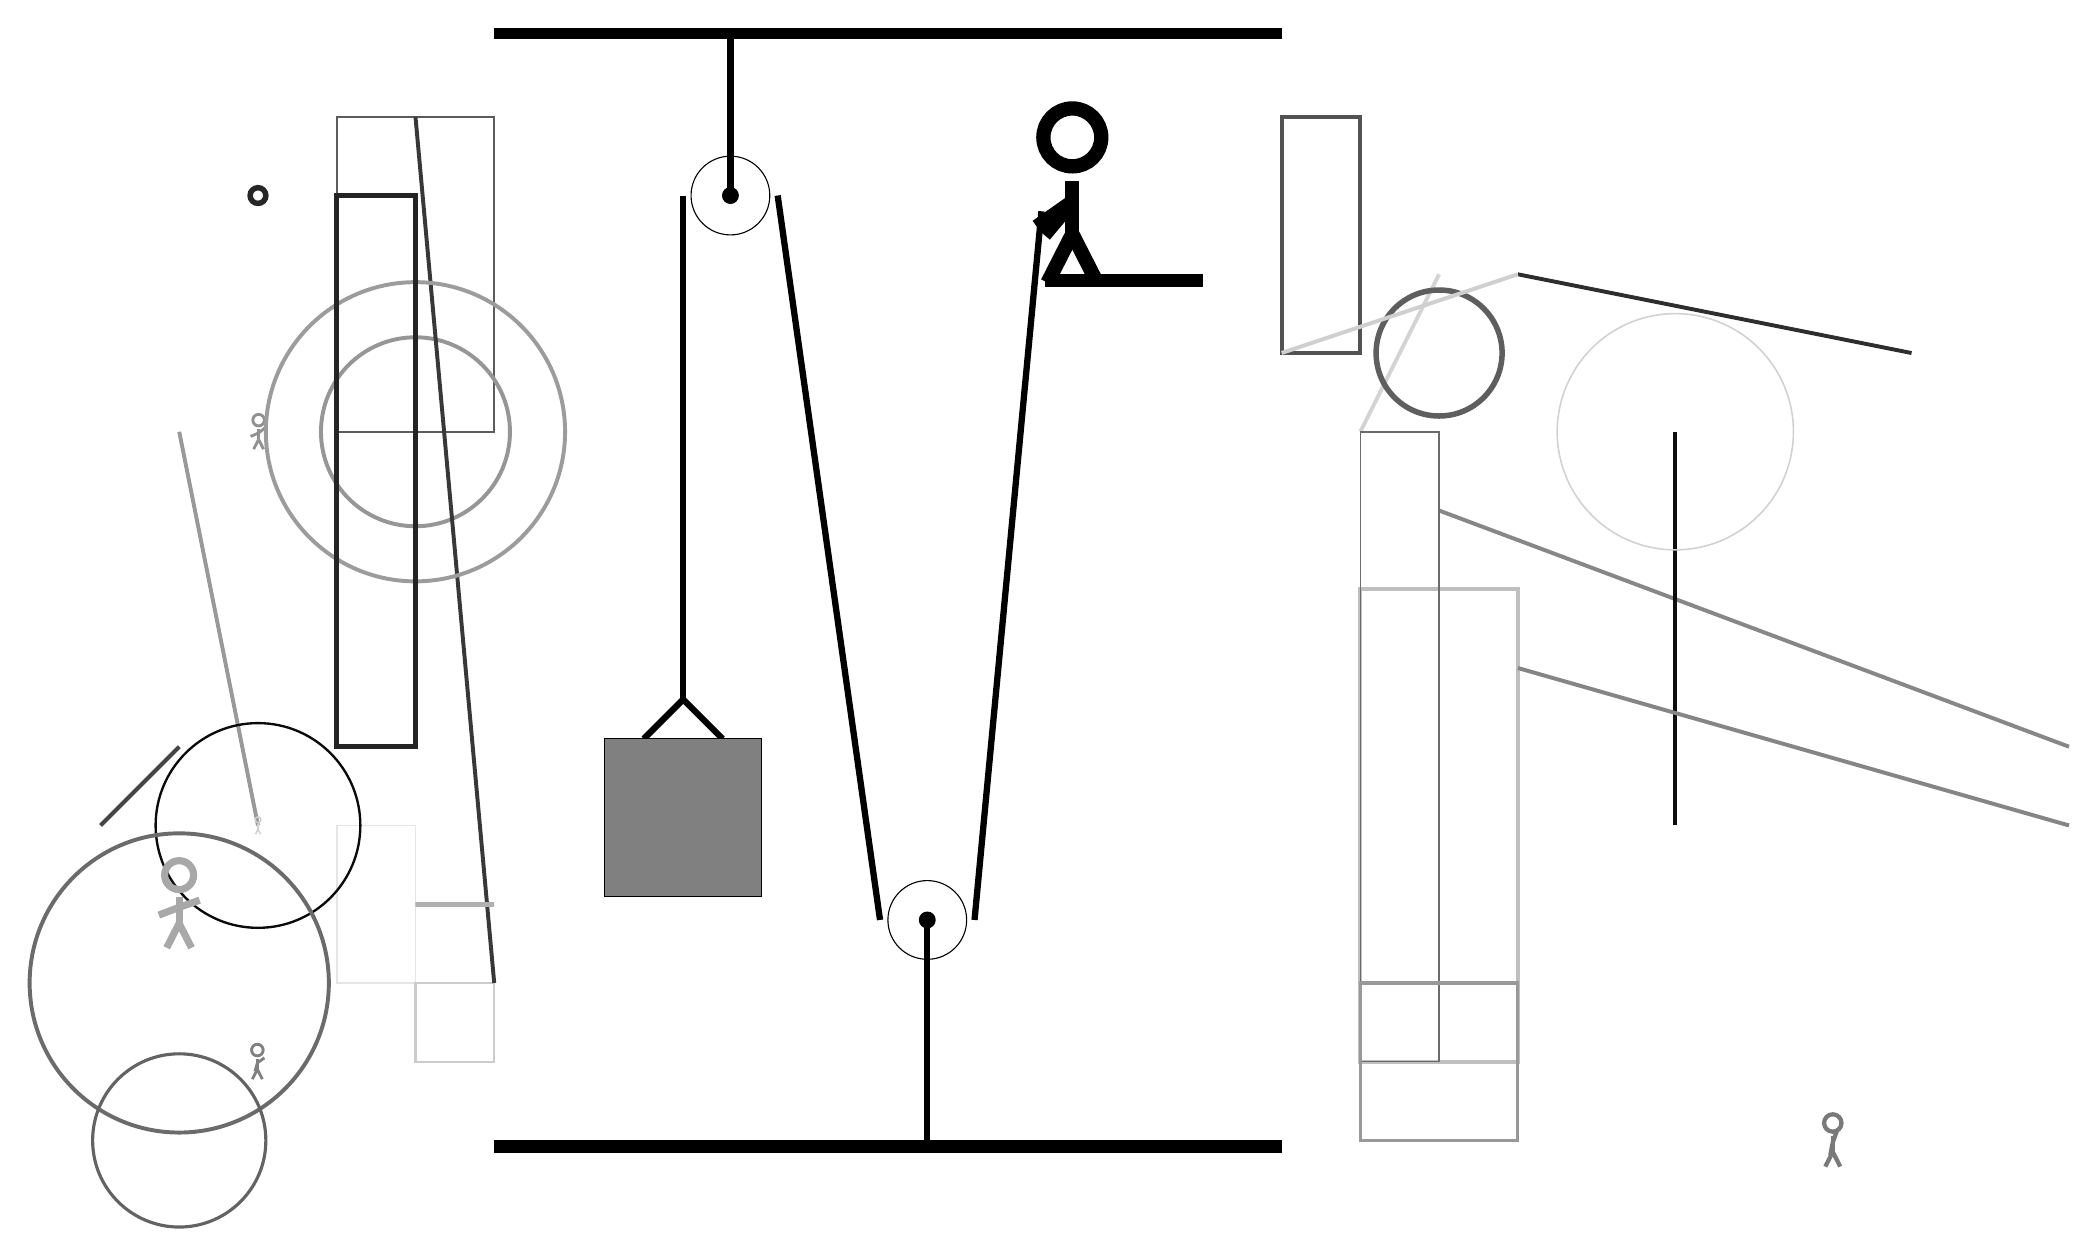
\begin{tikzpicture}
			%%%%% START %%%%%
			
			\draw[fill=black] (-2, 14) rectangle (8, 14.125);
			
			\draw (3.5, 2.8) circle (0.5);
			\draw[fill=black] (3.5, 2.8) circle (0.1);
			\draw[line width=0.8mm] (3.5, 2.8) -- (3.5, 0);
			
			\draw[line width=0.5mm, color=black!40](-6, 9) -- (-5, 4);
			
			\draw[line width=0.5mm, color=black!47](10, 8) -- (18, 5);
			\draw[line width=0.2mm, color=black!64] (-2, 9) rectangle (-4, 13);
			\draw[line width=0.5mm, color=black!17](9, 9) -- (10, 11);
			\draw[line width=0.2mm, color=black!10] (-3, 4) rectangle (-4, 2);
			
			\draw[line width=0.3mm, color=black!20] (-2, 1) rectangle (-3, 2);
			
			\draw [line width=0.3mm, color=black!96](-5, 4) circle (1.3);
			\draw[line width=0.5mm, color=black!68] (8, 10) rectangle (9, 13);
			\draw[line width=0.3mm, color=black!29] (10, 2) rectangle (10, 4);
			
			\node[line width=0.4mm, color=black!43] at (-5, 9) {\Strichmaxerl[2][23][39]};
			\draw [line width=0.5mm, color=black!41](-3, 9) circle (1.2);
			
			\draw[line width=0.5mm, color=black!95](13, 4) -- (13, 9);
			\draw[line width=0.5mm, color=black!82](11, 11) -- (16, 10);
			\draw[line width=0.5mm, color=black!25] (9, 7) rectangle (11, 1);
			\draw[line width=0.2mm, color=black!58] (10, 9) rectangle (9, 1);
			\node[line width=0.4mm, color=black!19] at (-5, 4) {\Strichmaxerl[1][83][72]};
			
			\draw[line width=0.4mm, color=black!40] (9, 0) rectangle (11, 2);
			
			\draw [line width=0.7mm, color=black!63](10, 10) circle (0.8);
			\node[line width=0.7mm, color=black!34] at (-6, 3) {\Strichmaxerl[5][21][19]};
			\draw[line width=0.5mm, color=black!78](-3, 13) -- (-2, 2);
			\node[line width=0.4mm, color=black!52] at (15, 0) {\Strichmaxerl[3][79][70]};
			
			\draw[line width=0.6mm, color=black!31] (-3, 3) rectangle (-2, 3);
			\draw[line width=0.5mm, color=black!19](11, 11) -- (8, 10);
			\draw[line width=0.5mm, color=black!73](-7, 4) -- (-6, 5);
			\draw [line width=0.2mm, color=black!18](13, 9) circle (1.5);
			
			\node[line width=0.4mm, color=black!50] at (-5, 1) {\Strichmaxerl[2][74][36]};
			
			\draw [line width=0.5mm, color=black!58](-6, 2) circle (1.9);
			\draw [line width=0.5mm, color=black!39](-3, 9) circle (1.9);
			\draw [line width=0.4mm, color=black!61](-6, 0) circle (1.1);
			
			\draw [line width=0.7mm, color=black!85](-5, 12) circle (0.1);
			\draw[line width=0.6mm, color=black!86] (-4, 12) rectangle (-3, 5);
			
			\draw[line width=0.5mm, color=black!48](11, 6) -- (18, 4);
			
			\draw (1, 12) circle (0.5);
			\draw[fill=black] (1, 12) circle (0.1);
			\draw[line width=0.8mm] (1, 14) -- (1, 12);
			
			\draw[line width=0.8mm](-0.1, 5.1) --  (0.4, 5.6) -- (0.9, 5.1);
			\draw[fill=black!50] (-0.6, 5.1) rectangle (1.4, 3.1);
			
			\draw[line width=0.8mm](0.4, 12) -- (0.4, 5.6);
			\centerarc[line width=0.8mm](1, 12)(180:0:0.6)
			\draw[line width=0.8mm](1.6, 12) -- (2.9, 2.8);
			\centerarc[line width=0.8mm](3.5, 2.8)(180:360:0.6)
			\draw[line width=0.8mm](4.1, 2.8) -- (4.95, 11.8);
			
			\node at (5.3, 12) {\Strichmaxerl[10][35][-130]};
			\draw[fill=black] (5, 11) rectangle (7, 10.85);
			
			\draw[fill=black] (-2, 0) rectangle (8, -0.15);
			
			%%%%% END %%%%%
		\end{tikzpicture}
	\end{figure}	
\end{document}